%
% front-black.tex -- template for standalon tikz images
%
% (c) 2020 Prof Dr Andreas Müller, Hochschule Rapperswil
%
\documentclass[tikz]{standalone}
\usepackage{amsmath}
\usepackage{times}
\usepackage{txfonts}
\usepackage{pgfplots}
\usepackage{csvsimple}
%\usepackage{geometry}
%\geometry{papersize={170mm,240mm},total={140mm,200mm},top=21mm,bindingoffset=10mm}

\usetikzlibrary{arrows,intersections,math}
\begin{document}
\def\skala{1}
\begin{tikzpicture}[>=latex,thick,scale=\skala]

\begin{scope}
\clip (23.0,2.1) rectangle (40.0,26.1);
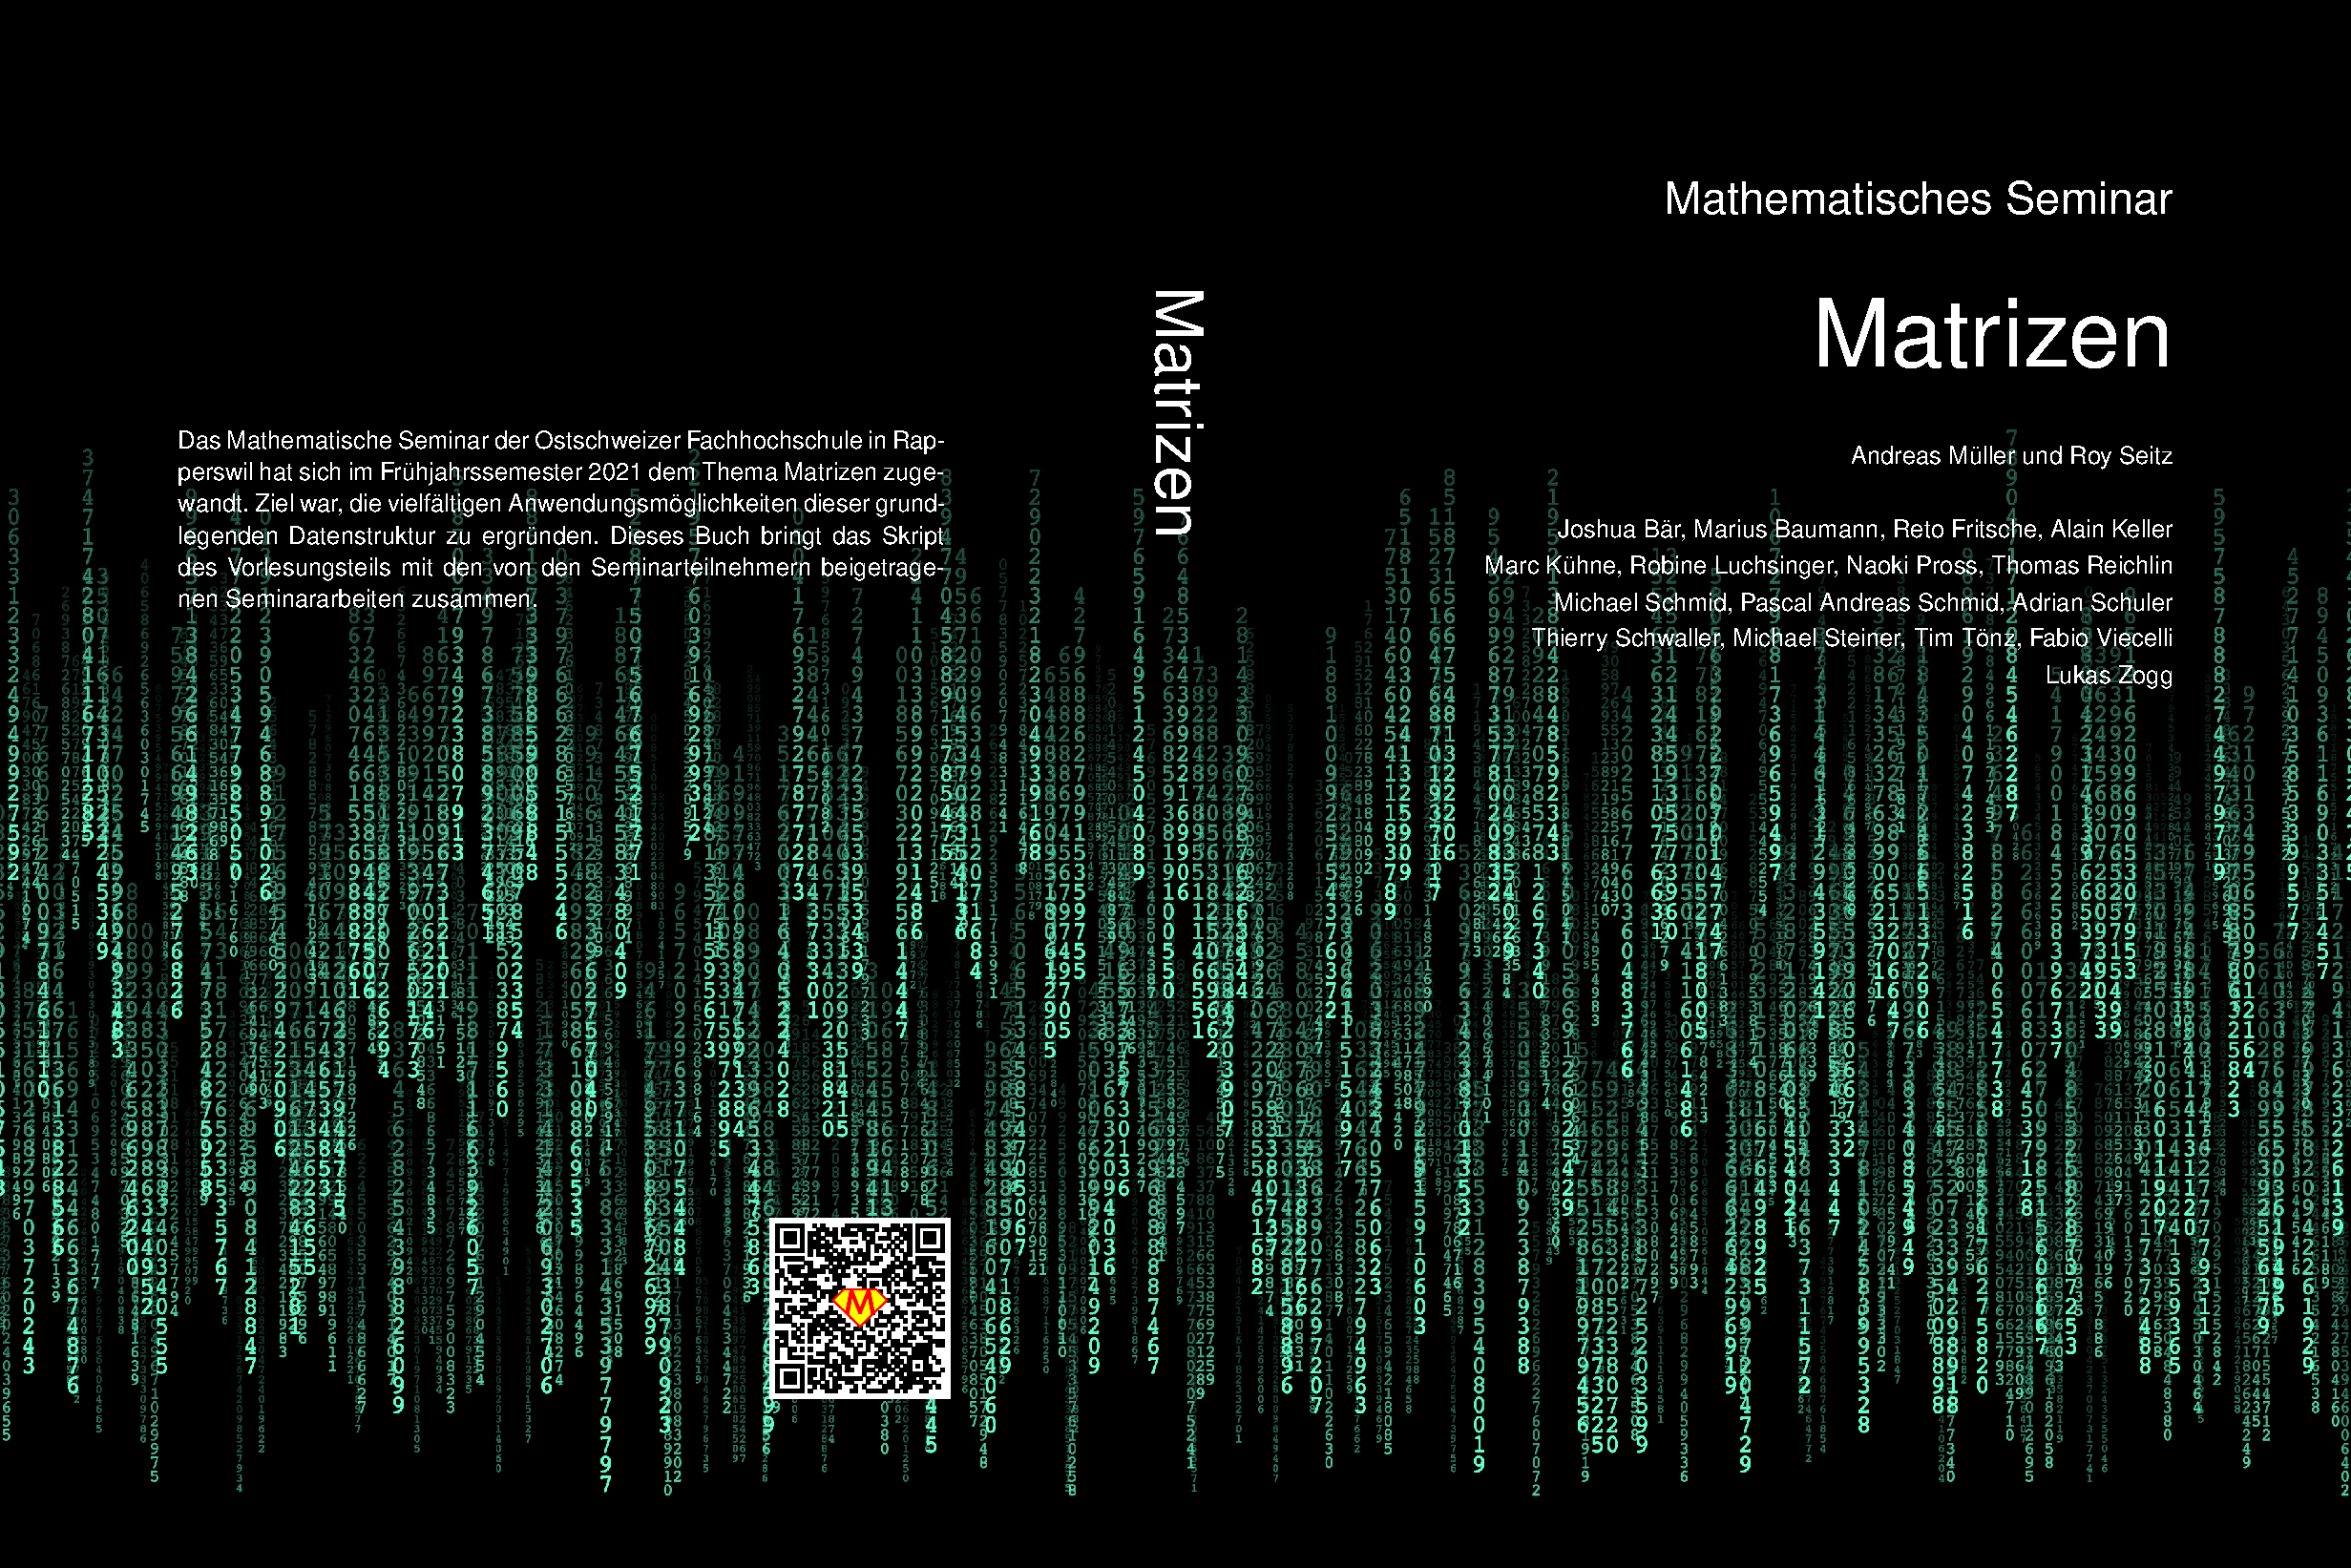
\includegraphics{buchcover-black.pdf}
\end{scope}

\end{tikzpicture}
\end{document}

